\section{Common losses and the joint load--cost set}
\label{sec:lossy}
With losses, early net grid energy no longer determines terminal purchases.
The same cardinality-matching values nevertheless suffice under the
common-window assumptions. Retaining finite cycling actions gives a complete
polygonal projection. Discarding dominated actions gives a smaller
\emph{efficient} frontier for monotone economic objectives. The two
descriptions have different economic and physical qualifications.

Retain the services, allowed graph, battery capacity $B$, positive fee $f$
and service-assigned buses of Section~\ref{sec:v2g}. Every bus starts and
finishes full, has zero reserve, and is available throughout the early
window. There is no travel, auxiliary consumption, taper or switching time.
Let $\alpha\in(0,1]$ be the common charging efficiency in both windows
and $\delta\in(0,1]$ the common discharging efficiency. Powers and energies
are measured on the \emph{grid side}: early purchases $C$ and exports $X$
use the shared connector's gross budget $C+X\le K$, and terminal grid
purchases satisfy $L\le H$. Each bus accepts the corresponding connector
power. Signed exports receive the same posted rate as purchases.
Write
\[
 S=\sum_i a_i+\sum_j b_j,\qquad P=\sum_i a_i,\qquad
 \kappa=\frac{1}{\alpha\delta}-1\ge0.
\]
Battery exchange is $\alpha C_v-X_v/\delta$, whereas net early grid
energy is $E=C-X$. Full replenishment gives
\begin{equation}\label{eq:lossyaccounting}
 L=\frac S\alpha-E+\kappa X.
\end{equation}
Thus two allocations with the same $E$ may have different $L$.
The supply objective must be defined on the resulting signed load domain,
or on an explicitly declared background-demand translation.

\subsection{The complete projection when finite cycling is allowed}
\label{sec:fulllossyprojection}
An exact projection can retain the otherwise dominated cycling actions.
We now explicitly permit any finite number of early charge/discharge
actions on a bus. There is no switching time, minimum session, separate
throughput fee, degradation cost or cycle limit. Common connector powers
are admissible in both directions for every bus, and all buses remain
available throughout the early window. Assume $B>0$ and a nonempty used
fleet. Economic objectives in this subsection depend on period-aggregate
loads and vehicle cost, rather than the timing or number of switches.
These assumptions are essential to the full-set claim.

\begin{theorem}[Complete common-loss load--cost projection]
\label{thm:fulllossyprojection}
For matching cardinality $m=0,\ldots,\nu$, let $N_m=2n-m$ and let
$r_m$ be the least total early battery requirement among allowed
matchings of size $m$. Define the compact polygon, possibly empty,
\begin{equation}\label{eq:fulllossypolygon}
\begin{split}
 W_m=\bigl\{(C,X):\;&C\ge r_m/\alpha,\quad X\ge0,\quad C+X\le K,\\
 &\max\{S-N_mB,S-\alpha H\}
       \le Q=\alpha C-X/\delta\le P\bigr\}.
\end{split}
\end{equation}
The complete physical load--cost projection is exactly
\[
 \bigcup_{m=0}^{\nu}
 \left\{\left(C-X,\frac{S-Q}{\alpha},fN_m\right):(C,X)\in W_m\right\}.
\]
Every point is attained by a finite-action schedule. Thus arbitrary
economic objective values on these projected quantities, including
negative posted-price value queries, are preserved without a monotonicity
assumption. Each nonempty polygon has at most five vertices; their affine
images generate the complete-plan convex hull with at most
$5(\nu+1)$ records, including lossless or lower-dimensional degeneracies.
\end{theorem}

\begin{proof}
Fix one matching, with fleet $N$, summed requirement $R$ and
$T=S-NB$. Let $x_v$ be a bus's net early battery increment.
Its paired, A-only and B-only endpoint boxes are respectively
\[
 [a_i+b_j-B,a_i],\qquad[a_i-B,a_i],\qquad[b_j-B,0].
\]
Their lower endpoints sum to $T$, their positive lower endpoints to $R$,
and their upper endpoints to $P$. Every upper endpoint is nonnegative.
Regardless of action order, $x_v=\alpha C_v-X_v/\delta$, so total
$Q\in[T,P]$. A positive lower endpoint requires at least its value
divided by $\alpha$ in purchases. Hence $C\ge R/\alpha$ is necessary.
The other inequalities are nonnegative exports, shared gross use and
full-terminal accounting $L=(S-Q)/\alpha\le H$. Terminal purchases are
nonnegative because $Q\le P<S$; individually each box upper endpoint
also leaves a nonnegative refill requirement.

Conversely fix aggregate totals satisfying these inequalities with $R$
in place of $r_m$. For any $Q\in[T,P]$, the boxes admit an exchange
vector whose positive parts sum to $A=\max\{R,Q\}$. If $Q\ge R$,
start from positive lower endpoints and zero elsewhere, distributing
$Q-R$ through the remaining headrooms. If $Q<R$, keep mandatory positive
increments and distribute negative increments of total $Q-R$ through the
negative lower intervals, whose combined lower endpoint is $T-R$.
One-direction exchanges then realize
\[
 C_0=A/\alpha,\qquad X_0=\delta(A-Q).
\]
Since $X\ge0$ implies $\alpha C\ge Q$, and
$\alpha C\ge R$, we have $z=C-C_0\ge0$ and
$X-X_0=\alpha\delta z$.

Realize these residuals by battery-neutral cycles on one existing bus
before its one-direction exchange. At early SOC $s\in[0,B]$, use
charge-then-discharge cycles of depth at most $B-s$ if $s\le B/2$,
and discharge-then-charge cycles of depth at most $s$ otherwise.
The permitted depth is at least $B/2>0$. Split the residual battery
throughput $\alpha z$ into finitely many such chunks, allowing a smaller
last chunk. Each returns to $s$, stays in $[0,B]$, and uses grid purchases
depth$/\alpha$ and exports $\delta$ times depth. Their total residual
is exactly $(z,\alpha\delta z)$, with no limiting or Zeno argument.

Execute the cycles and then all one-direction exchanges serially.
Their gross grid throughput is exactly $C+X\le K$, so they fit the
common early window at the admitted power. Endpoint boxes ensure
subsequent service feasibility; nonnegative service consumption preserves
intermediate SOC. Refill serially at the terminal, using total
$L\le H$. If $K=0$, all early actions are zero and no positive-power
division is required. If $H=0$, only zero terminal amounts could be
admitted; under the present positive B-service energies, $P<S$ makes
every polygon empty, consistently with physical infeasibility.

At fixed $m$, only $R$ depends on the matching: $S,P,N,T$ and the fee
are constant. Its entire polygon is contained in the polygon for a
matching attaining $r_m$, and every point of that larger polygon has
just been physically constructed. This proves exact equality of the
union, not merely economic dominance. Equation~\eqref{eq:fulllossypolygon}
has five halfspaces in the plane. Its bounded polygon has at most five
vertices; affine images and then finite convex combinations prove the
generator claim. When $\alpha\delta=1$, the map collapses to
$E+L=S/\alpha$ rather than being invertible; the same argument still
applies.
\end{proof}

\begin{corollary}[Capped identical idle buses in the complete projection]
Under the same zero-transition model, permitting identical paid idle buses
with a total fleet cap $2n$ leaves this complete projection unchanged.
\end{corollary}
An idle bus has exchange box $[-B,0]$. A fleet with matching size $m$ and
$q$ idle buses has $q\le m$ by the cap. Delete $q$ matching edges and
serve their services separately. This preserves total $N,S,P,T$ and fee,
while lowering $R$. The resulting all-assigned polygon reproduces the same
$C,X,Q,E,L,c$, including cycles. Reverse inclusion is immediate. Identical
access, efficiency, capacity and fees are required; nonzero transition
consumption would change $S$ under deletion and needs a separate argument.

Let $V$ be the vertex-image records in the theorem. An exact continuous
formulation for complete-plan convexification is the familiar relation
\[
 \operatorname{conv}\mathcal P
   =\left\{\sum_{v\in V}\lambda_vv:
          \lambda_v\ge0,\ \sum_{v\in V}\lambda_v=1\right\},
\]
where $\mathcal P$ denotes the complete projected set above. A convex
$F$ gives ordinary convex planning on each polygon and on this hull;
physical planning takes the minimum over the cardinalities. These are
standard convex-optimization tools. Merely interpolating $r_m$ at a
fractional cardinality and substituting into physical inequalities is
not this disjunctive hull construction and remains unjustified.

Removing a neutral cycle keeps $Q,L$ fixed and lowers $E$ by
$(1-\alpha\delta)z$. This explains why monotone objectives can discard
it in the efficient-frontier result below, while arbitrary objectives
must retain the full polygons. Its smaller set $Z$ still requires the
stated monotonicity assumptions. The finite cycle count can be large;
no runtime or generic hull-algorithm claim is made. A separate eight-case
exact qualification of these full polygons, described in
Appendix~\ref{app:evidence}, includes finite-action physical replay.
It supplies no public-timetable V2G, empirical or learning evidence.
The earlier one-direction qualification has a different scope.

\paragraph{Why a negative-price query needs the full set.}
Take $n=1$, $B=1$, $a=b=3/4$, $\alpha=1/2$, $\delta=1$,
$K=2$, $H=3$ and $f=2$. At the fixed posted prices $p=(-3,1)$,
the private score is $c-3E+L$. For the paired one-bus assignment,
\[
 C=11/6,\quad X=1/6,\quad Q=3/4,
 \qquad (E,L,c)=(5/3,3/2,2)
\]
gives score $-3/2$. This point has a finite physical realization.
After A the battery holds $1/4$: purchase $1/3$ grid units and export
$1/6$, returning to $1/4$, then purchase $3/2$ to reach full.
These three early actions have gross energy 2 and serialize at power 2
within the early window. B leaves $1/4$; terminal purchases $3/2$
restore full inventory within the power-3 terminal window.

This is the exact response value, not just a feasible score.
For $m=1$, the polygon has $C\ge1$ and
$1/2\le C/2-X\le3/4$; for $m=0$, it has $C\ge0$ and
$0\le C/2-X\le3/4$. Both impose $X\ge0$ and $C+X\le2$.
Their scores are respectively $5-4C+5X$ and $7-4C+5X$.
For any feasible $C$, use the smallest export
$X=\max\{0,C/2-3/4\}$. The resulting score decreases on both
pieces, with final endpoint $C=11/6$, giving minima $-3/2$ and
$1/2$, respectively. Thus the complete-fleet response value is $-3/2$.

The efficient curves instead have $L=3-E$: the two-bus curve has
$0\le E\le3/2$, $c=4$, and the one-bus curve has
$1\le E\le3/2$, $c=2$. Their best scores are 1 and $-1$.
Discarding the neutral cycle therefore changes this query's value from
$-3/2$ to $-1$. It raises early purchases without changing terminal
refill, so the negative early rate rewards a point that monotone
economics discards. Because the queried objective is linear, its minimum
over the physical set and its complete-plan hull is the same:
$D=\CH=-3/2$ for this objective. This is not a positive planning gap
or an equilibrium claim. This analytical anchor also passed the separate
full-polygon implementation control; it gives no public-timetable V2G conclusion.

\begin{figure}[htbp]
\centering
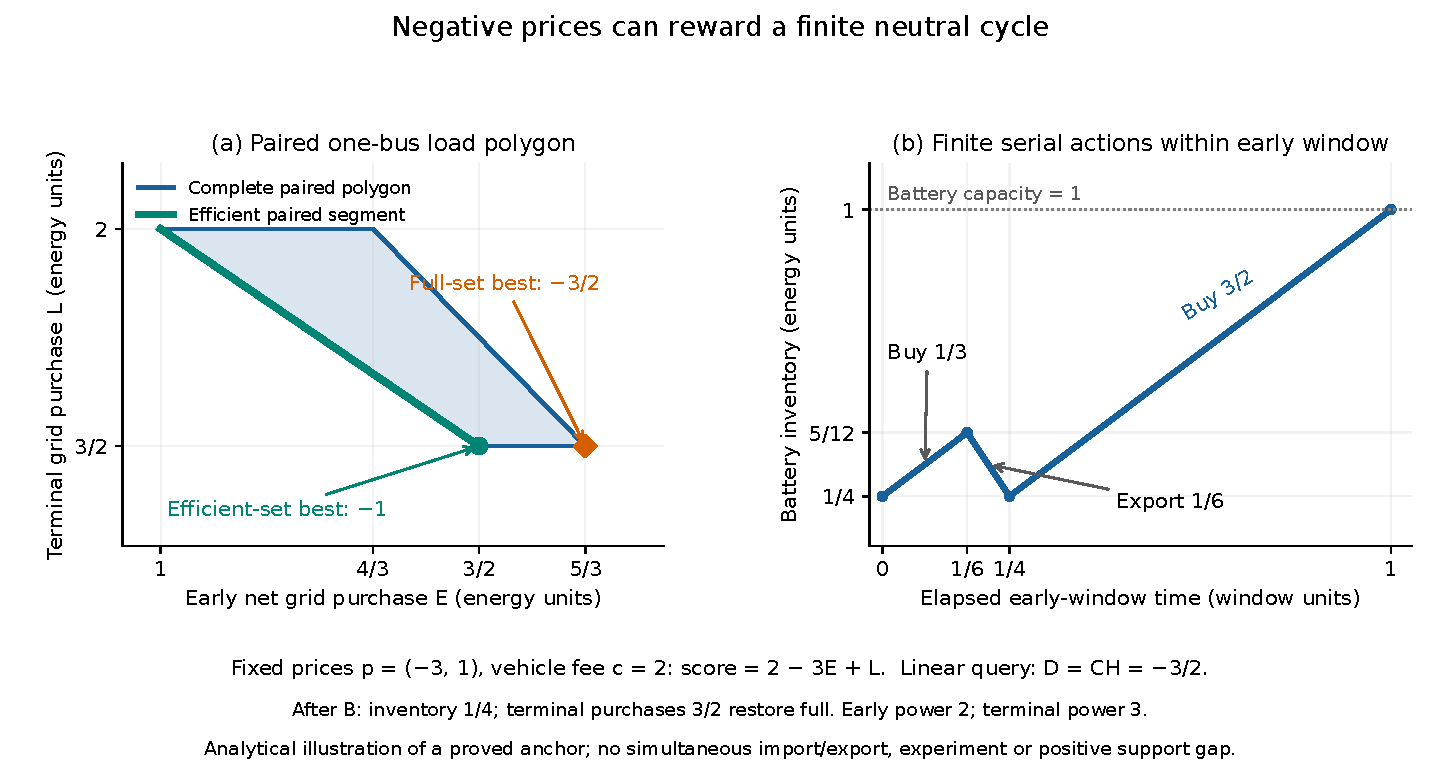
\includegraphics[width=\textwidth]{figures/full_lossy_polygon-v2.pdf}
\caption{The full paired polygon retains a finite neutral cycle that the
efficient frontier discards. At the negative posted price, that cycle improves
the fleet's linear response value. This illustration has $D=\CH$; it is not a
positive planning-gap example. The right panel shows the three serial early
actions of the same physical witness.}
\label{fig:fullpolygon}
\end{figure}

\begin{corollary}[Directional powers, affine wear and a finite action cap]
\label{cor:directionalwear}
Retain the full-action assumptions of
Theorem~\ref{thm:fulllossyprojection}. In the unit early window let common
purchase power be $K_c>0$ and export power $K_d>0$, accepted by every
bus in the corresponding direction. Replace the gross-budget halfspace by
\[
 C/K_c+X/K_d\le1.
\]
With the other four halfspaces unchanged, these are still the exact
cardinality polygons. For common affine grid-throughput wear coefficients,
their complete joint load--cost images are
\[
 E=C-X,\qquad L=(S-Q)/\alpha,\qquad
 c=fN_m+w_cC+w_dX+w_tL.
\]
Each polygon still has at most five vertices, whose affine images generate
the complete-plan hull. Fixed nonnegative wear coefficients have their
usual cost interpretation; exact projection equality itself needs no
coefficient-sign or economic-monotonicity restriction.

For a fixed used fleet $N$, every attainable aggregate point has a
realization with at most
\[
 N+2\left\lceil\frac{2\alpha K_c}{B}\right\rceil
 \quad\hbox{early charge/export actions},\qquad
 N\quad\hbox{terminal charge actions}.
\]
An action cap at least these bounds preserves the aggregate projection,
not every literal schedule. Replacing $N$ by $2n$ gives one bound for
all cardinalities under the standing fleet cap.
\end{corollary}

\begin{proof}
The endpoint boxes, mandatory purchases and terminal accounting are
unchanged. Necessity of the new halfspace follows because the two
directions occupy at least $C/K_c$ and $X/K_d$ connector time and cannot
overlap. For sufficiency use the same baseline exchanges and neutral
cycles as in Theorem~\ref{thm:fulllossyprojection}. Execute each purchase
at power $K_c$ and each export at $K_d$; their total serial duration is
exactly the displayed occupancy. Directional asymmetry adds no SOC
condition. At fixed cardinality a minimum-$R$ matching reproduces the
same $C,X,Q,L$, hence the same affine wear cost, for any other matching.
This proves complete-set equality; affine imaging and convex combination
give the vertex and hull claims. The common-task version uses $S_m$
in place of $S$, as in Corollary~\ref{cor:commontransitionfull}.

The residual $z=C-C_0$ has battery throughput $\alpha z\le\alpha K_c$.
Choosing chunks of depth $B/2$, with a possibly smaller last chunk, needs at most
$J=\lceil2\alpha K_c/B\rceil$ cycles, each with two actions. The chosen
orientation fits the bus's initial SOC, and each cycle returns to it.
Each bus then needs at most one baseline early action and one terminal
charge; zero actions are omitted. Restricting to this action count adds
no aggregate point and removes none, since every point has the explicit
bounded-action realization. The count is conservative, not minimal,
and does not bound runtime or the number of actions in arbitrary schedules.
\end{proof}

Wear must remain in the cost image. In the lossless case a neutral cycle
adds equal amounts $z$ to $C,X$, leaving $E,L$ unchanged but adding
$(w_c+w_d)z$ to intrinsic cost. Thus net loads and a constant vehicle
fee alone cannot represent this complete joint projection. For the same
reason, convexification retains each component's actual wear cost. Affine
wear commutes with averaging when $C,X,L$ remain separate; mean net loads
alone need not determine it.

This corollary does not transfer the smaller efficient-$Z$ formulas to
unequal powers or wear, nor cover SOC/depth/rate-dependent degradation,
per-session cost, positive switching time, minimum durations or
heterogeneous acceptance. Its positive-power assumptions are separate
from the theorem's zero-budget cases. It is an analytical extension with
no numerical implementation qualification: the eight full-polygon cases
use symmetric early powers and no wear. No public-timetable, empirical
wear-calibration or computational-advantage conclusion follows.


\subsection{The smaller efficient frontier for monotone costs}

\begin{lemma}[Least terminal purchase at a fixed early net load]
\label{lem:lossyfixed}
Fix an allowed matching $M$ of size $m$, using $N=2n-m$ buses. Put
\[
 R=\sum_{(i,j)\in M}[a_i+b_j-B]_+,\quad T=S-NB,\quad
 d_R(E)=\left[\frac R\alpha-E\right]_+,\quad
 L_R(E)=\frac S\alpha-E+\kappa d_R(E).
\]
Among early allocations with at most one direction of action per bus,
the feasible early-net interval is exactly $[t(R,N),U]$, when nonempty,
where
\begin{align}
 U&=\min\{P/\alpha,K\},\label{eq:lossyU}\\
 t(R,N)&=\max\left\{
 (1/\alpha-\delta)R+\delta(S-NB),\quad
 2R/\alpha-K,\quad S/\alpha-H,\quad
 \frac{S/\alpha+\kappa R/\alpha-H}{1+\kappa}
 \right\}.\label{eq:lossyt}
\end{align}
For each such $E$, the least attainable terminal purchase is $L_R(E)$.
It is achieved with $C=E+d_R(E)$ and $X=d_R(E)$.
\end{lemma}

The first threshold in \eqref{eq:lossyt} accounts for available battery
inventory; the second prevents offsetting purchases and exports from
evading connector time. The last two enforce terminal refill on both
pieces of $L_R$. In particular, replacing service energy by $S/\alpha$
in the lossless formula would omit both the export loss and its connector
consequences.

Retain the allowed-graph matching values $r_m$ from
Section~\ref{sec:heterogeneous}, for $m=0,\ldots,\nu$. Define
$N_m=2n-m$, $t_m=t(r_m,N_m)$, $L_m=L_{r_m}$ and $c_m=fN_m$.
\begin{theorem}[Finite efficient-frontier reduction with common losses]
\label{thm:lossyfrontier}
The set
\begin{equation}\label{eq:lossyZ}
 Z=\bigcup_{\substack{0\le m\le\nu\\t_m\le U}}
 \{(E,L_m(E),c_m):t_m\le E\le U\}
\end{equation}
is physical. Every physical point is weakly dominated coordinatewise
in $(E,L,c)$ by a point of $Z$ with the same operating cost. Hence the
complete physical set's coordinatewise efficient frontier is obtained
by removing dominated points from $Z$. The thresholds $t_m$ are
nondecreasing and discretely convex.

Each cardinality contributes at most two line segments, with a possible
kink at $E=r_m/\alpha$. Thus $\operatorname{conv}Z$ is the convex hull
of finitely many segment endpoints and kinks. If the convex supply
objective is coordinatewise nondecreasing on the admitted signed domain,
physical and hull planning values can be computed over $Z$ and
$\operatorname{conv}Z$, respectively, without changing either value.
\end{theorem}

Dominance here allows a replacement with smaller early load as well as
smaller terminal load; it does not identify the full physical set.
Under nonnegative early and terminal posted prices, the same reduction
preserves the minimum bill plus operating cost. At zero prices dominated
allocations can tie, so it does not enumerate every price response.
Negative prices or a nonmonotone supply objective may require the alternatives
retained by Theorem~\ref{thm:fulllossyprojection}; they cannot use the smaller
set $Z$ by assertion. Asymmetric export settlement must keep its distinct
purchase/export coordinates. The lossless scalar criterion
for the location of a supported hull optimum is not asserted here:
different cardinalities can have different terminal loads at the same $E$.
Convex network dispatch with increasing generation costs need not give a
load-monotone value function: congestion can make a nodal marginal price
negative. Appendix~\ref{app:networkmonotonicity} gives an exact illustration
and the established pricing precedent. The smaller efficient set therefore
requires a load-domain monotonicity check. The complete polygons instead
retain all period-aggregate load/cost points, subject to their explicit
cycling assumptions and the network objective's declared domain.

Identical paid idle buses remain redundant for these efficient values
under the total fleet cap $2n$. Deleting as many matching edges as there
are idle buses preserves the total fleet and fee and lowers $R$, so an
all-assigned fleet has no larger $L$ at the same $E$. This efficient-set
argument gives dominance. If finite cycling is retained, the complete
projection result above gives the stronger equality of the whole projected
set, as its capped-idle corollary explains.
There is no general uncapped-idle conclusion when negative net early loads
are valuable. The theorem remains conditional on common efficiencies,
common windows and ideal serial use; it is not a public-timetable V2G
result. A separate ten-case exact qualification matched these formulas to
independent raw SOC/sign-polytope enumeration, checking every physical
vertex and attainment along complete frontier segments. These finite
implementation checks supplement the proof; they do not establish
empirical validity or prevalence.

\subsection{Planning and support from the finite frontier}
\label{sec:lossyalgorithm}
The reduction gives a direct way to compute the two planning values under
the monotonicity assumptions of Theorem~\ref{thm:lossyfrontier}. There are
at most $2(\nu+1)$ affine segments and $M\le3(\nu+1)$ generating records
$v_j=(u_j,c_j)$, where $u_j=(E_j,L_j)$; empty intervals are omitted and
singletons require only one record. Physical planning minimizes
$c_m+F(E,L_m(E))$ on each segment, a convex one-dimensional problem,
and takes the smallest value. Hull planning solves
\[
 \min_{\lambda\ge0,\;\sum_j\lambda_j=1}
 \left\{\sum_j\lambda_jc_j+
 F\!\left(\sum_j\lambda_ju_j\right)\right\}.
\]
These use standard matching and convex-optimization tools; the physical
result is that the matching values suffice to construct their input.

\begin{remark}[Interpolate complete plans, not fractional fleet physics]
\label{rem:fractionalcardinality}
Interpolating $r_m$ and substituting a continuous cardinality into
\eqref{eq:lossyt} need not give this hull. Take one service per batch,
$B=1$, $a=b=3/4$, $\alpha=1/2$, $\delta=1$, $K=2$, $H=3$ and $f=2$.
Then $r_0=0$, $r_1=1/2$; the two complete efficient branches are
\[
 (E,3-E,4),\quad 0\le E\le3/2;\qquad
 (E,3-E,2),\quad 1\le E\le3/2.
\]
Both physical and hull minima of $c+3E+L$ equal $7$. Instead put
$r(m)=m/2$, $N=2-m$ and $c=2N$ for fractional $m$. The same formulas
admit $m=1/2$, $E=1/4$, $L=3$, $c=3$, of cost $27/4<7$:
the four lower bounds in \eqref{eq:lossyt} are $1/4,-1,0,1/4$,
and the terminal formula gives $3$. Every actual mixture with mean
cardinality $m$ requires $E\ge m$, so this point is fictitious.
Taking maxima of resource bounds after averaging can relax the averages
of complete feasible branches. Convexity of the matching sequence proves
neither equality nor physical attainability of that shortcut. The finite
generator formulation above retains the required coupling exactly.
This example has no true physical--hull gap: the artificial reduction
creates one.
\end{remark}

For differentiable $F$, a proposed hull point
$(\bar u,\bar c)=\sum_j\lambda_j(u_j,c_j)$ has a short sufficient
certificate: feasible weights, its exact objective and gradient
$p=\nabla F(\bar u)$, and the inequalities
\[
 c_j+p\cdot u_j\ge\bar c+p\cdot\bar u
 \qquad\text{for every generating record }j.
\]
Convexity proves optimality on the hull; nonnegative $p$ and physical
dominance extend the private-score lower bound to all original plans.
For any nonnegative posted price, the minimum private score is likewise
the minimum over these records. At zero prices this computes the value,
not every response: discarded dominated plans or entire segments can tie.

If the generators and convex quadratic coefficients are rational, there
exists a hull optimum with rational loads, cost and weights, permitting
an exact rational certificate. Rational physical data, including the
efficiencies, suffice for rational generators; a rational objective alone
does not. At any optimum the supporting functional has normal $(p,1)$,
so its face has dimension at most two, or the whole hull already does.
Thus at most three generators suffice. Enumerating their simplex faces
and solving rational linear stationarity systems also handles singular
positive-semidefinite quadratics; no inverse of a singular Hessian is
required. Flat optimum sets can contain irrational points despite the
existence of a rational representative. These finite deductions make no
new runtime or general scheduling-complexity claim.

% Parent may invoke this macro in the appendix after inputting this file.
\newcommand{\LossyProjectionProofs}{%
\section{Proofs for the common-loss efficient projection}\label{app:lossy}
\begin{proof}[Proof of Lemma~\ref{lem:lossyfixed}]
In battery coordinates $x_v$, the boxes are
$[a_i+b_j-B,a_i]$ for a paired bus, $[a_i-B,a_i]$ for an A-only bus,
and $[b_j-B,0]$ for a B-only bus. Their positive lower endpoints sum
to $R$, all lower endpoints to $T$, and upper endpoints to $P$.
Available negative battery exchange therefore totals $R-T$.
A one-direction allocation has
$C_v=(x_v)_+/\alpha$ and $X_v=\delta(-x_v)_+$.
Mandatory purchases give $C\ge R/\alpha$, hence
$X=C-E\ge d_R(E)$. Equation~\eqref{eq:lossyaccounting} proves the
terminal lower bound.

For $E\ge R/\alpha$, use no negative exchange and distribute positive
battery exchange $\alpha E$ among the independent intervals, whose
positive totals fill $[R,P]$. For $E<R/\alpha$, keep mandatory positive
coordinates at their lower bounds and distribute negative battery
exchange $(R/\alpha-E)/\delta$ over the negative intervals. This is
possible exactly when
$E\ge R/\alpha-\delta(R-T)$.
These constructions attain $d_R(E)$ and span the raw interval
$[(1/\alpha-\delta)R+\delta T,P/\alpha]$.
For any one-direction allocation the same endpoints are necessary from
$C\ge R/\alpha$, $X\le\delta(R-T)$ and $C\le P/\alpha$.

The construction's gross grid throughput is
$E+2d_R(E)=\max\{E,2R/\alpha-E\}$, the minimum possible at that $E$.
The early constraint is therefore exactly $E\le K$ and
$E\ge2R/\alpha-K$. Also
\[
 L_R(E)=\max\{S/\alpha-E,
 S/\alpha+\kappa R/\alpha-(1+\kappa)E\}.
\]
Requiring both pieces to be at most $H$ gives the last two bounds in
\eqref{eq:lossyt}. Each early action is monotone between valid endpoint
inventories and can be serialized; each terminal refill is between zero
and $B/\alpha$ grid units and all refills serialize when their sum is
at most $H$. Zero-power cases require zero energy without division.
This proves necessity and physical attainment. The curve is strictly
decreasing in $E$, so its distinct points at the same fee do not dominate
one another.
\end{proof}

\begin{proof}[Proof of Theorem~\ref{thm:lossyfrontier}]
At a fixed cardinality, every term of $t(R,N)$ and $L_R(E)$ is
nondecreasing in $R$. A matching attaining $r_m$ therefore has a
feasible interval containing that of any other matching of the same
size, and a terminal load no larger at the same early load and fee.
The lemma gives the physical replacement. Standard cardinality-matching
convexity applies to $r_m$. Its linear interpolation, multiplied by
nonnegative constants and combined with the affine nondecreasing term
$\delta(S-(2n-m)B)$, shows that every threshold component is convex
and nondecreasing. Their maximum has these properties, hence its integer
samples $t_m$ do as well.

A bus with purchases and exports can have a battery-neutral cycle
removed: reduce $C_v$ by $\varepsilon$ and $X_v$ by
$\alpha\delta\varepsilon$, until one is zero. Battery exchange and
terminal load are unchanged, while connector use and early net purchase
weakly decrease. Reconstructing a monotone action in the common window
preserves inventory feasibility. Removing all such cycles and applying
the preceding matching replacement gives a point of $Z$ weakly below
every physical point, with unchanged fee. Conversely every point of $Z$
is physical. Removing dominated points from $Z$ therefore yields exactly
the physical efficient frontier.

The displayed $L_m$ has at most one kink, giving the finite-segment and
convex-hull description. For a coordinatewise nondecreasing supply
objective, replacement cannot worsen physical cost. Replacing each
component of an arbitrary whole-plan mixture similarly lowers its mean
load coordinatewise without changing its mean operating cost, so it
cannot worsen hull cost. The reverse inequalities follow from physical
inclusion of $Z$. This proves equality of the reduced values.

For $k$ capped paid idles, the fleet has size $N=2n-m+k\le2n$, hence
$k\le m$. Delete $k$ matching edges; the resulting all-assigned fleet
has the same $N$ and fee, no larger $R$ and the same $T=S-NB$.
The same replacement argument proves the stated efficient-value
redundancy, without asserting equality of all projected loads.
\end{proof}
}
